% TEXINPUTS=.:$HOME/git/bvtex: latexmk  -pdf ggd.tex


\documentclass[10pt,xcolor=dvipsnames]{beamer}
\input{defaults}

\input{beamer/preamble}
\usepackage[outline]{contour}

\definecolor{bvtitlecolor}{rgb}{0.98, 0.92, 0.84}
\definecolor{bvoutline}{rgb}{0.1, 0.1, 0.1}

\newcommand{\worch}{\textit{worch}\xspace}
\newcommand{\waf}{\textbf{waf}\xspace}

\renewcommand{\bvtit}{GeGeDe}
\renewcommand{\bvtitle}{\LARGE \textcolor{DarkOrchid}{General Geometry Description\\The \texttt{gegede} Package}}
\renewcommand{\bvevent}{}
\renewcommand{\bvbeamerbackground}{}

\begin{document}
\input{beamer/title.tex}
\input{beamer/toc.tex}

\section{Introduction}

\begin{frame}
  \frametitle{In a Nutshell}

  \textbf{Ge}neral \textbf{Ge}ometry \textbf{De}scription:\footnote{GeGeDe or GGD.  Pronounce it however you wish.}
  \vspace{-5mm}
  \begin{center}
    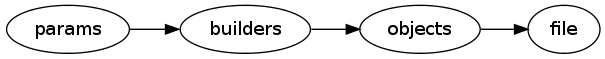
\includegraphics[width=0.8\textwidth]{highlevel.pdf}
  \end{center}
  \vspace{-5mm}
  \begin{itemize}
  \item Simple \textbf{pipeline} of geometry information processing.
  \item Uses a simple system for \textbf{authoring} geometry descriptions.
  \item Authors write the description using a mix of:
    \begin{itemize}
    \item A simple configuration language (\textbf{params})
    \item Structured Python code (\textbf{builders})
    \end{itemize}
  \item Produces in-memory \textbf{objects} adhering to a \\ \textit{Constructive Solid
    Geometry} (CSG) schema,
  \item Which are finally \textbf{exported} to variety of formats.
  \end{itemize}

\end{frame}

\begin{frame}
  \frametitle{Non-features}
  GeGeDe is focused on authoring.  Non-features include:
  \vspace{5mm}
  \begin{itemize}
  \item[$\times$] \textbf{No tracking} or other geometry querying algorithms.  
    \begin{itemize}\footnotesize
    \item[$\times$] It is \textbf{not} a replacement for
      \href{https://geant4.web.cern.ch/}{Geant4}, nor ROOT's
      \href{https://root.cern.ch/root/html/GEOM_GEOM_Index.html}{TGeo/GEOM}
    \item[\checkmark] But, it can produce geometry data for them.
    \end{itemize}
  \item[$\times$] \textbf{No geometry content validation}, eg overlapping volumes.
    \begin{itemize}\footnotesize
    \item[\checkmark] But, other apps can check the exported geometry.
    \item[\checkmark] And, it will assure valid output formats.
    \item[?] Trivial hooks exist to add content validation in the future.
    \end{itemize}
  \item[$\times$] \textbf{No built-in visualization} services.
    \begin{itemize}\footnotesize
    \item[\checkmark] But, some of its formats can be visualized by other applications.
    \end{itemize}
  \item[$\times$] \textbf{No interactive/GUI} for model editing. It is not CAD.
    \begin{itemize}\footnotesize
    \item[\checkmark] But, has some experimental export format support for \href{https://www.freecadweb.org/}{FreeCAD}
    \end{itemize}
  \end{itemize}
\end{frame}

\section{Software Design}
\begin{frame}
  \tableofcontents[currentsection,hideothersubsections]
\end{frame}

\begin{frame}
  \frametitle{Design Overview}

  \vspace{-5mm}
  \begin{center}
    \includegraphics[width=0.8\textwidth]{layers.pdf}
  \end{center}
  \vspace{-5mm}

  \begin{description}
  \item[params] High-level, human-centric configuration language.
    \begin{itemize}\scriptsize
    \item[-] Provided by experiment s/w developers, fiddled with by end users.
    \end{itemize}
  \item[builders] Structured, procedural geometry construction code.
    \begin{itemize}\scriptsize
    \item[-] Experiment developers write this code.
    \end{itemize}
  \item[objects] In-memory representation of full geometry.
    \begin{itemize}\scriptsize
    \item[-] Following strict schema defined in GeGeDe.
    \end{itemize}
  \item[export] Conversion to format suitable for some application.
    \begin{itemize}\scriptsize
    \item[-] Batteries included with GeGeDe, or user-provided modules.
    \end{itemize}
  \end{description}
\end{frame}

\subsection{Configuration}

\begin{frame}[fragile]
  \frametitle{Configuration}
\small
\begin{verbatim}
[everything]  
class = mymodule.mybuilders.WorldBuilder
subbuilders = ["farsite", "nearsite", "testhall"]
size = Q("1000km")

[farsite]
class = mymodule.mybuilders.SiteBuilder
subbuilders = ["lardet"]
wireangle = Q("35*deg")
# etc, ...
\end{verbatim}

  \begin{itemize}\footnotesize
  \item Each section binds \textbf{name} and \textbf{parameter set} to a \textbf{builder instance}.
  \item One special builder provides the ``world'' logical volume.
    \begin{itemize}\scriptsize
    \item File can configure multiple world builders.
    \item First one listed ``wins'', or can specify one on the command line.
    \end{itemize}
  \item The \texttt{class} and \texttt{subbuilders} are the only reserved keys.
    \begin{itemize}\scriptsize
    \item The only two keywords reserved by GeGeDe internals.
    \item Builders are free to require any additional key/value pairs (\textit{eg}. \texttt{size, wireangle}).
    \end{itemize}
  \item Use \texttt{Q("...")} for expressing units\footnote{\url{http://pint.readthedocs.org/}} (\texttt{Q} short for ``quantity'').
  \end{itemize}

\end{frame}

\subsection{Builders}

\begin{frame}[fragile]
  \frametitle{Builders - GeGeDe's main code structure}
  \begin{itemize}
  \item Builders written as \textbf{experiment-provided} code:
    \begin{itemize}\footnotesize
    \item It does not ``live'' in the \texttt{gegede} Git repo!
    \item Builders are subclasses of \texttt{gegede.builder.Builder} (or suitably duck-typed)
    \end{itemize}

  \item Each builder:
    \begin{itemize}\footnotesize
    \item Responsible for constructing some portion of the geometry.
    \item Exposes zero or more logical volume (LV) objects to the \textbf{parent builder}.
    \item Properly places the LVs of its \textbf{daughter builders} (\textit{subbuilders}) into its own LVs.
    \end{itemize}
    
  \item Builders typically are written as a \textbf{cooperative hierarchy}:
    \begin{itemize}\footnotesize
    \item Builders can delegate to subbuilders.
    \item Explicit subbuilder creation is allowed but better
      flexibility is achieved by listing then with the
      \texttt{subbuilders} configuration keyword.
    \item Typically follow a loosely-coupled design but
      some collusion or ``software contract'' can be useful.
    \item Arbitrary complex builder associations are allowed.  A
        1-parent/$n$-children tree is common.
    \end{itemize}



  \end{itemize}

\end{frame}

\begin{frame}[fragile]
  \frametitle{Example Builder Hierarchy}
  \vspace{-5mm}
  \begin{center}
    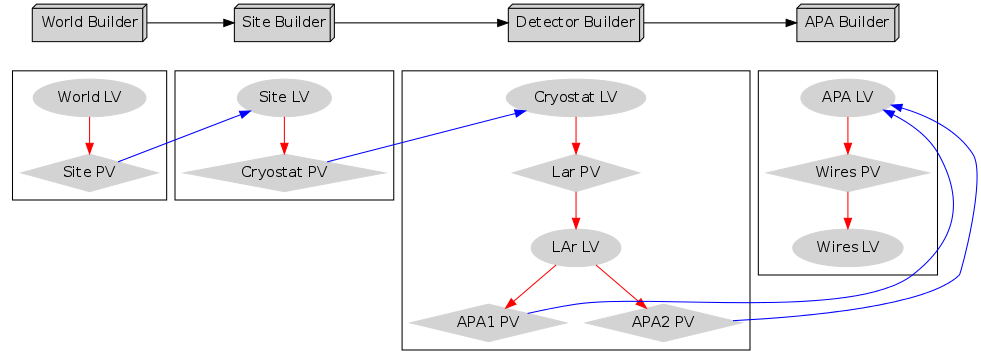
\includegraphics[width=0.8\textwidth]{buildhier2.pdf}    
  \end{center}
  \vspace{-5mm}
  
  \begin{itemize}\footnotesize
  \item \textbf{Factor} each builder based on \textbf{geometry symmetries}.
  \item Builders directly construct ``local'' geometry.
  \item Hierarchy design best to follow loosely-coupled software contract:
    \begin{itemize}\scriptsize
    \item Child builder \textbf{exposes} select LV(s) such that,
    \item Parent builder knows how/where to \textbf{place} them.
    \end{itemize}
  \item Allows for:
    \begin{itemize}\scriptsize
    \item Decoupled development and reuse of builders.
    \item Test ``worlds'' narrowed to a subbuilder's exposed LVs
    \end{itemize}
  \end{itemize}
\end{frame}

\begin{frame}[fragile]
  \frametitle{Builder Code Example}

  \footnotesize

  \begin{lstlisting}[language=Python]
class MyBuilder(gegede.builder.Builder):

  def configure(self, dx='1m', dy='2m', dz='3m', **kwds):
    # Receive user configuration, providing defaults.
    # Incompatible units are caught as errors.
    # Here, configure self, in some way.
    self.size = (dx,dy,dz)

  def construct(self, geom):
    # Do local construction using ``geom'' object as only interface.
    box = geom.shapes.Box(self.name+'_shape', *self.size)
    # Add ``top-level'' LV to .volumes list for our parent to use.
    self.add_volume(box)   
    # Place LVs from our child builders, guaranteed already constructed.
    for sb in self.builders:
      for sv in sb.volumes:
        # ... place ``sv'' in ``box'' ...
  \end{lstlisting}

\end{frame}

\subsection{Objects}

\begin{frame}
  \frametitle{Geometry Objects} 

  GeGeDe objects follow the CSG model:
  \begin{description}
  \item[shapes] (aka ``solids'') such as box, tubs, sphere, etc
  \item[matter] elements, isotopes, mixtures, materials, etc
  \item[structure] rotations, positions, logical and physical volumes
  \end{description}

  These objects:
  \begin{itemize}
  \item Reference each other by name to form some graph.
    \begin{itemize}\footnotesize
    \item Name-based references used to parallel GDML's schema.
    \item May explicitly name objects or GeGeDe will generate a unique name.
    \end{itemize}
  \item Are represented as Python \texttt{namedtuple} instances.
  \item Objects follow a specific
    \href{https://github.com/brettviren/gegede/blob/master/python/gegede/schema/__init__.py}{schema}
  \end{itemize}
\end{frame}

\begin{frame}[fragile]
  \frametitle{Schema Definition Language} 
  \begin{lstlisting}[language=Python]
Schema = dict(
  shapes = dict(
    Box = (("dx","1m"), ("dy","1m"), ("dz","1m")),
    # ...
  matter = dict(
    Element = (("symbol",str), ("z",int), ("a","0.0g/mole")),
    # ...
  structure = dict(
    Placement = (("volume", Named), ("pos", Named), ("rot", Named)),
    # ...
  \end{lstlisting}

  \footnotesize
  \begin{itemize}
  \item Schema written simply as a static Python data structure
    \begin{itemize}\scriptsize
    \item[-] (link to \href{https://github.com/brettviren/gegede/blob/master/python/gegede/schema/__init__.py}{\texttt{gegede.schema.Schema}})
    \end{itemize}
  \item Follows naming and function prototype conventions of Geant4 geometry construction methods.
    
  \item Linear dimensions are usually taken as ``half lengths'' (eg, \texttt{dx})
  \item Attributes defined as \texttt{(name, type)} pair.  The type is either a
    Python type object or a string that evaluates to a \texttt{pint.Quantity} unit object and which provides a default value.
    \item Weakly typed references to other objects via \texttt{gegede.types.Named} type.
  \end{itemize}
\end{frame}


\subsection{Export}

\begin{frame}
  \frametitle{Exporters}

  Exporters produce persistent representations of GeGeDe objects.

  \vspace{5mm}

  Some export formats supported by GeGeDe are:

  \begin{description}
  \item[GDML] for Geant4.  Uses \texttt{lxml.etree} for assuring valid XML.
  \item[ROOT] direct \texttt{TGeo} object creation (requires PyROOT)
  \item[JSON] trivial dump preserving GeGeDe internal object schema.
  \item[OIV] OpenInventor SceneGraph 
  \end{description}

  \vfill

  New exporters should be easy to develop.
  \begin{itemize}\footnotesize
  \item Depends on the format, of course.
  \item Developing and testing the GDML exporter took about 2 hours.
  \item The JSON one took about 2 minutes! 
    \begin{itemize}\tiny
    \item[:)] It's a ``cheat'' as it just uses \texttt{json.dumps()}!
    \end{itemize}
  \end{itemize}

  \vfill

  GeGeDe supports exporters as independent Python modules.
  \begin{itemize}\footnotesize
  \item Contributions back to GeGeDe are welcome!
  \end{itemize}
\end{frame}

\section{Usage}
\begin{frame}
  \tableofcontents[currentsection,hideothersubsections]
\end{frame}

\begin{frame}[fragile]
  \frametitle{Installation}
  GeGeDe requires:
  \begin{itemize}
  \item Python 2.7/3.5+
  \item Pint (for units)
  \item LXML (XML support)
  \item PyROOT (optional)
  \end{itemize}

  \vfill

  Install from source:
\begin{verbatim}
$ git clone https://github.com/brettviren/gegede.git
$ cd gegede/
$ python setup.py install
\end{verbatim}

  \vfill

  Install from PyPI:
\begin{verbatim}
$ pip install gegede
\end{verbatim}
\end{frame}

\begin{frame}[fragile]
  \frametitle{Interfaces}
  Command line:
\begin{verbatim}
$ gegede-cli -h
usage: gegede-cli [-h] [-w WORLD] [-f FORMAT] [-o OUTPUT] 
                  [-V] [-O] [-F]
                  [-d DOT_FILE] [-D DOT_HIERARCHY]
                  config [config ...]
\end{verbatim}

  \vfill

  In principle can be used as module in a larger application by understanding: 
  \begin{lstlisting}[language=Python]
    gegede.main.main()
  \end{lstlisting}
  
\end{frame}

\begin{frame}
  \frametitle{Documentation}

  \begin{center}
    Documentation starts with the main \texttt{README} on GitHub:

    \vspace{1cm}

    \url{https://github.com/brettviren/gegede/}    
  \end{center}

\end{frame}

\section{Status}

\begin{frame}
  \tableofcontents[currentsection,hideothersubsections]
\end{frame}


\begin{frame}
  \frametitle{GeGeDe Status}
  \begin{itemize}
  \item Main users now are doing DUNE Near Detector design studies.
    \begin{itemize}\footnotesize
    \item They got up to speed using GeGeDe very quickly.
    \item New users are welcome.  You don't have to study neutrinos! :)
    \end{itemize}
  \item Fairly stable code:
    \begin{itemize}\footnotesize
    \item[\checkmark] No open issues in the GitHub project!
      \begin{itemize}\scriptsize
      \item[$\sim$] GDML export is best supported, others may have hiccups.
      \end{itemize}
    \item[\checkmark] Recent contributions from DUNE (J. Palomino) adding more shapes
      \begin{itemize}\scriptsize
      \item[$\times$] Still need a few more for have 100\% coverage of all Geant4 shapes!
      \end{itemize}
    \item[\checkmark] Python 3.5+ support \textbf{just} added.
      \begin{itemize}\scriptsize
      \item[$\sim$] Maybe some 2.7'isms still left uncovered.
      \end{itemize}
    \end{itemize}
  \item I'll continue to support GeGeDe at the level of bug fixes.
    \begin{itemize}\footnotesize
    \item[:)] Major new features will likely be accepted but let's
      talk first.
    \end{itemize}
  \end{itemize}

\end{frame}


\end{document}

